\documentclass[aspectratio=169]{beamer}
\usetheme{Madrid}
\usecolortheme{whale}

\usepackage{fontspec}
\setsansfont{Arial}
\setmainfont{Times New Roman}
\usepackage[vietnamese]{babel}
\usepackage{graphicx}
\usepackage{booktabs}

\title[GreenLab realtime]{Xử lý dữ liệu quan trắc thời gian thực GreenLab}
\date{20/06/2026}

\begin{document}

\begin{frame}\titlepage\end{frame}

\begin{frame}{Nội dung}\tableofcontents\end{frame}

% ===================================================================
\section{Bối cảnh \& Mục tiêu}
\begin{frame}{Bối cảnh \& Mục tiêu}
  \begin{itemize}
    \item Dự án bổ sung nguồn \textbf{dữ liệu thời gian thực GreenLab} (IoT, $\sim$3--5 phút/lần, MongoDB Atlas).
    \item \textbf{4 trạm}, mỗi trạm 5 cảm biến: COD, NH4, pH, nhiệt độ, TSS. Hiện chỉ trạm \textbf{Cát Bà (HP)} có dữ liệu (15.475 bản ghi).
    \item \textbf{Thách thức:} mô hình phân loại cần \textbf{19 chỉ số} (cá giò HP) -- \textbf{21 chỉ số} (hàu QN), cảm biến chỉ cấp 5.
    \item \textbf{Mục tiêu:} (1) giám sát QCVN-10; (2) suy ra đủ chỉ số để phân loại phù hợp.
  \end{itemize}
\end{frame}

% ===================================================================
\section{Dữ liệu}
\begin{frame}{Dữ liệu: 23 ngày, 1 trạm, 5 cảm biến}
  \begin{columns}
    \begin{column}{0.54\textwidth}
      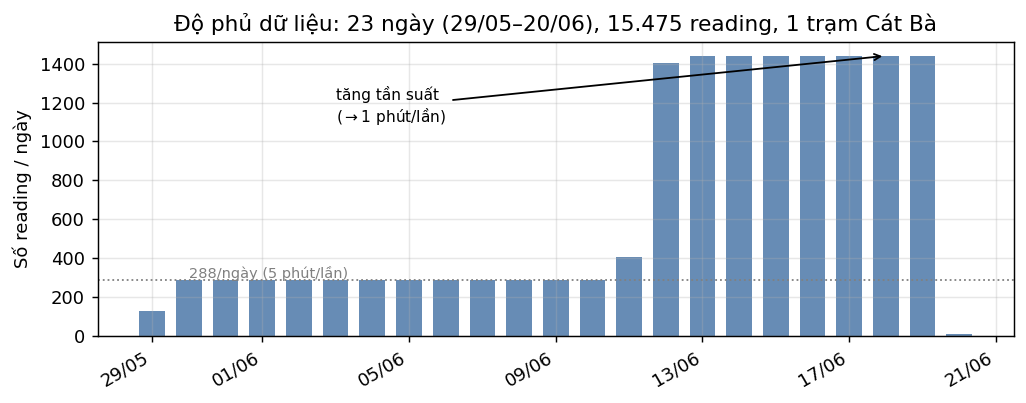
\includegraphics[width=\linewidth]{../figures/data_coverage.png}
    \end{column}
    \begin{column}{0.46\textwidth}
      \footnotesize
      \textbf{15.475 reading}, 29/05--20/06.
      \begin{itemize}\small
        \item Tần suất 5 phút $\to$ \textbf{1 phút} từ 12/06 (nửa sau dày $\sim$5$\times$).
        \item COD trung vị $=558{,}8 =$ max $\Rightarrow$ kẹt trần.
        \item NH4 thô 77--160 (lệch cao).
        \item pH/Temp ổn định; TSS lệch phải.
      \end{itemize}
    \end{column}
  \end{columns}
\end{frame}

\begin{frame}{Phân phối giá trị 5 cảm biến}
  \begin{center}
    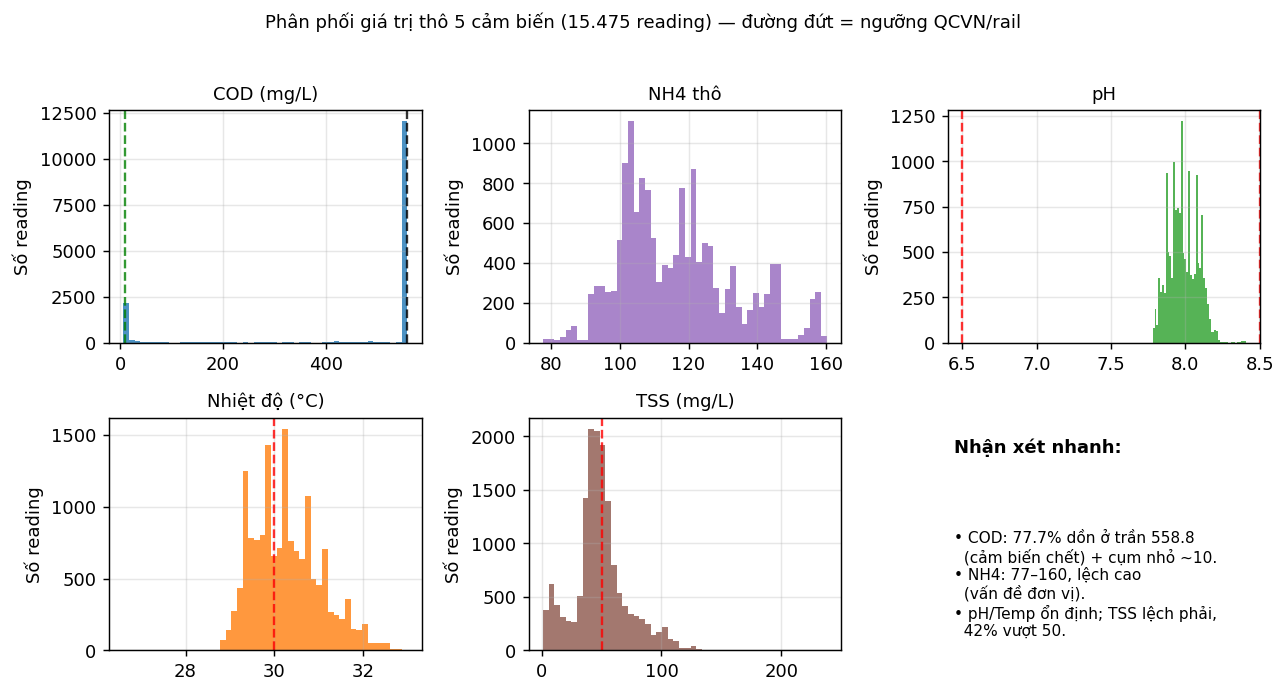
\includegraphics[height=0.72\textheight]{../figures/value_dist.png}
  \end{center}
  \footnotesize Ba vấn đề lộ ngay: COD lưỡng đỉnh dồn trần; NH4 lệch cao (đơn vị); TSS 42\% vượt 50.
\end{frame}

% ===================================================================
\section{Phát hiện dữ liệu}
\begin{frame}{Phát hiện 1: cảm biến COD đã chết}
  \begin{columns}
    \begin{column}{0.46\textwidth}
      \begin{itemize}\small
        \item Phẳng $\sim$10 mg/L tới 05/06.
        \item Trôi tăng 06--10/06 (28$\to$452).
        \item Kẹt cứng trần \textbf{558{,}8} từ 11/06.
        \item 77{,}7\% bản ghi $=558{,}8$, phương sai 0.
        \item $\Rightarrow$ \textbf{bão hòa cảm biến}, không phải ô nhiễm. Cần vệ sinh đầu dò.
      \end{itemize}
    \end{column}
    \begin{column}{0.54\textwidth}
      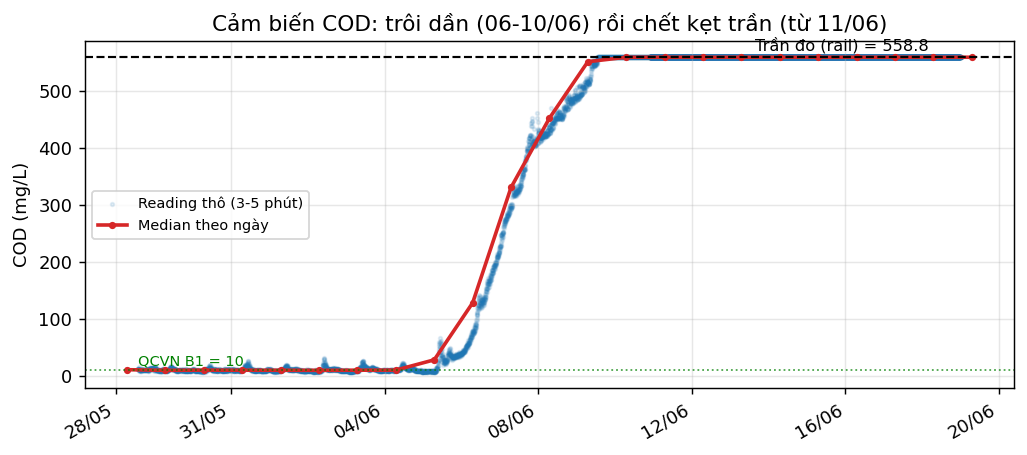
\includegraphics[width=\linewidth]{../figures/cod_timeline.png}
    \end{column}
  \end{columns}
\end{frame}

\begin{frame}{Phát hiện 2: đơn vị NH4 + hóa học NH3}
  \begin{itemize}
    \item NH4 thô 77--160 --- nếu mg/L thì vô lý; khả năng cao $\mu$g/L ($\div1000\approx$ ngưỡng QCVN 0{,}1).
    \item Cảm biến đo \textbf{NH4$^+$} (ít độc); QCVN đánh giá \textbf{NH3} (rất độc) --- không map thẳng.
    \item Quy đổi Emerson theo pH + nhiệt độ:
      \[ \text{NH3} = \text{NH4}_{\text{raw}}\cdot s\cdot \frac{1}{1+10^{(pK_a-pH)}} \]
    \item Đơn vị lật kết luận: $s{=}0{,}001\to$ NH3 0{,}0077 (đạt); $s{=}1\to$ 7{,}66 (vượt 76$\times$). $\Rightarrow$ tham số hóa + in rõ giả định.
  \end{itemize}
\end{frame}

% ===================================================================
\section{Phương pháp}
\begin{frame}{Xử lý theo nhóm: cascade 4 tầng lấp 19--20 chỉ số}
  \begin{center}\small
  \begin{tabular}{clc}
    \toprule
    \textbf{Tầng} & \textbf{Chỉ số / cách lấy} & \textbf{Độ tin} \\
    \midrule
    1 & \textbf{Đo trực tiếp}: pH, nhiệt độ, TSS (+COD khi QC đạt) & cao nhất \\
    2 & \textbf{Suy hóa học}: NH3 (NH4 + pH + Temp qua Emerson) & cao \\
    3 & \textbf{Nội suy ML}: DO, Salinity, PO4, BOD5, Transparency, Alkalinity & tùy $R^2$ \\
    4 & \textbf{Mặc định trung vị}: kim loại nặng, Coliform, H2S, COD\dots & thấp nhất \\
    \bottomrule
  \end{tabular}
  \end{center}
  \vspace{4pt}\footnotesize
  Ưu tiên từ trên xuống: đo thật $\to$ hóa học $\to$ ML $\to$ trung vị.
  \par\vspace{2pt}\textbf{Ghi chú:} DO + độ muối (trọng số 1\&2) không đo trực tiếp được nhưng \emph{nội suy được} (mức mạnh).
\end{frame}

\begin{frame}{Pipeline 8 module}
  \begin{center}\small
  \texttt{fetch} $\to$ \texttt{quality} (QC) $\to$ \texttt{chemistry} (NH3) $\to$
  \texttt{monitor} $\to$ \texttt{impute} $\to$ \texttt{classify} $\to$ \texttt{report}
  \end{center}
  \begin{itemize}
    \item \textbf{QC:} lọc dòng ngoài dải + phát hiện rail/flatline (loại COD 558{,}8).
    \item \textbf{Nội suy thích nghi theo VÙNG:} train riêng HP-only (cá giò) + QN-only (hàu);
      mỗi vùng 2 bộ \textbf{5f/4-feature} thích nghi theo COD. QC chọn bộ + vùng.
    \item \textbf{3 mức tin cậy:} $R^2\ge0{,}4$ ML-mạnh · $0{,}2$--$0{,}4$ ML-yếu (cờ) · $<0{,}2$ median; artifact loại.
    \item \textbf{Phân loại:} ghép đủ chỉ số $\to$ chấm điểm breakpoint chuyên gia.
  \end{itemize}
\end{frame}

\begin{frame}{Mô hình nội suy: học từ data thật, đoán chỉ số thiếu}
  \begin{center}
    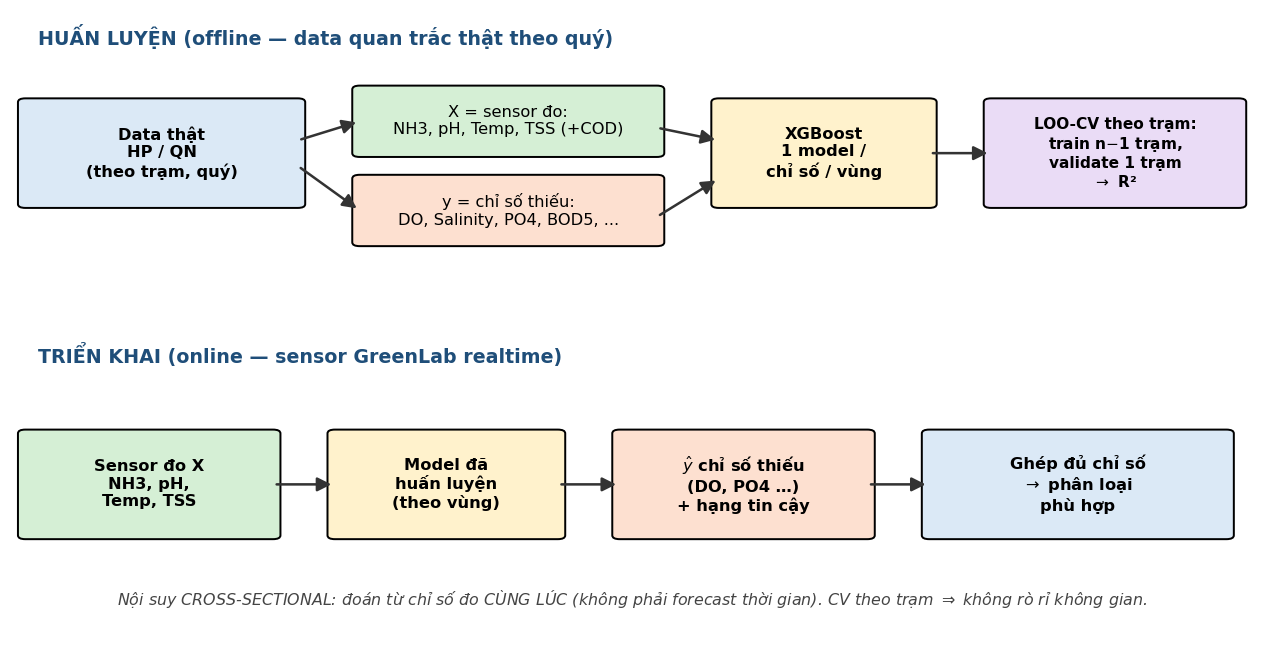
\includegraphics[width=0.95\linewidth]{../figures/impute_method.png}
  \end{center}
  \vspace{-4pt}\footnotesize
  \textbf{Huấn luyện:} đầu vào X = chỉ số sensor đo (NH3, pH, Temp, TSS, +COD); đầu ra y = chỉ số thiếu.
  XGBoost 1 model/chỉ số/vùng, kiểm định \textbf{LOO-CV theo trạm} (train n$-$1 trạm, validate trạm còn lại). \textbf{Triển khai:} sensor đo X $\to$ model $\to$ $\hat{y}$ $\to$ phân loại.
\end{frame}

\begin{frame}{Hai luồng xử lý độc lập ở bước nội suy}
  \begin{columns}
    \begin{column}{0.5\textwidth}
      \footnotesize
      \textbf{Luồng 1 --- theo trạng thái COD:}
      \begin{itemize}\small
        \item COD VALID $\to$ \textbf{5-feat} (cắt dòng COD lỗi).
        \item COD INVALID $\to$ \textbf{4-feat} (rớt COD, không bịa median).
      \end{itemize}
      \vspace{4pt}
      \textbf{Luồng 2 --- theo vùng huấn luyện:}
      \begin{itemize}\small
        \item \textbf{HP-only}: cùng vịnh, DO đoán được.
        \item HP+QN gộp: nhiều mẫu nhưng khác chế độ $\to$ phá DO.
      \end{itemize}
    \end{column}
    \begin{column}{0.5\textwidth}
      \centering\footnotesize
      \begin{tabular}{lcc}
        \toprule
        & 5-feat & 4-feat \\ \midrule
        \textbf{HP-only} & 5 cột$^*$ & \textbf{Cát Bà 20/06} \\
        HP+QN & 5 cột & 4 cột \\
        \bottomrule
      \end{tabular}
      \par\vspace{6pt}\scriptsize
      Thực thi chọn ô theo (vùng $\times$ COD QC).\\[2pt]
      $^*$HP không có cột COD $\Rightarrow$ ``5-feat'' thực chất 4 cột (\texttt{feat\_cols.json}).
    \end{column}
  \end{columns}
\end{frame}

% ===================================================================
\section{Kết quả}
\begin{frame}{Kết quả 6 chỉ số nội suy --- chính sách 3 mức}
  \begin{columns}[T]
    \begin{column}{0.55\textwidth}
      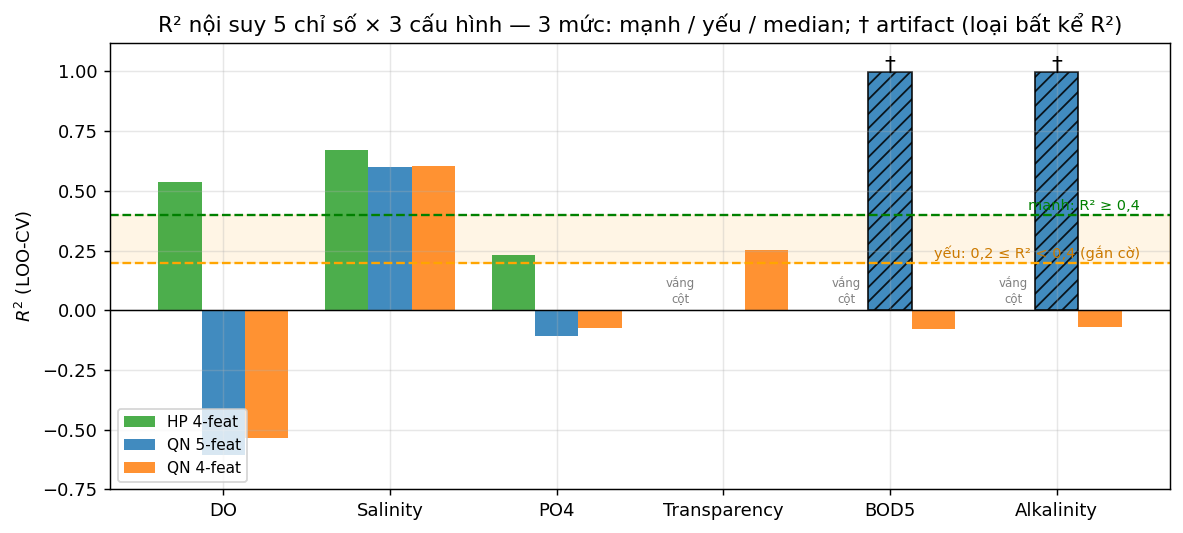
\includegraphics[width=\linewidth]{../figures/r2_all.png}
    \end{column}
    \begin{column}{0.45\textwidth}
      \scriptsize
      \begin{tabular}{lccl}
        \toprule
        Chỉ số & HP & QN (5f/4f) & Hạng \\
        \midrule
        \textbf{DO}       & \textbf{0{,}54} & $-0{,}61$/$-0{,}54$ & \textbf{mạnh} \\
        \textbf{Salinity} & \textbf{0{,}67} & $0{,}60$/$0{,}60$ & \textbf{mạnh}$\times$2 \\
        PO4               & 0{,}23 & $-0{,}11$/$-0{,}07$ & \textbf{yếu} (HP) \\
        Transp.           & --- & $-0{,}00$/$0{,}25$ & \textbf{yếu} (QN) \\
        BOD5              & --- & $0{,}99^\dagger$/$-0{,}08$ & artifact \\
        Alkal.            & --- & $1{,}00^\dagger$/$-0{,}07$ & artifact \\
        \bottomrule
      \end{tabular}
      \par\vspace{4pt}\scriptsize
      mạnh $\ge0{,}4$ · yếu $0{,}2$--$0{,}4$ (cờ) · $<0{,}2$ median.\\
      $\dagger$ artifact $\to$ loại bất kể R².\\[3pt]
      \footnotesize\textbf{2 mạnh (DO, Salinity) + 2 yếu.}
    \end{column}
  \end{columns}
\end{frame}

\begin{frame}{Vì sao chỉ Salinity, không phải kim loại? --- bằng chứng}
  \begin{center}
    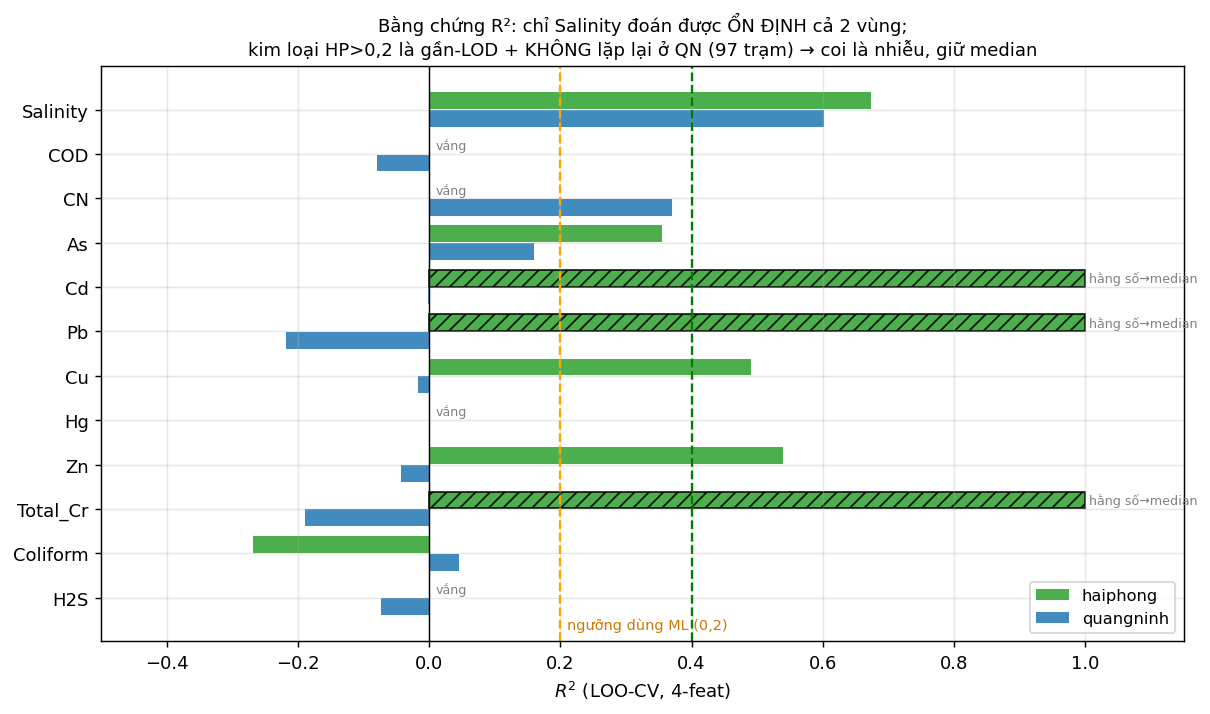
\includegraphics[height=0.72\textheight]{../figures/median_params_r2.png}
  \end{center}
  \footnotesize Đã test ML cho \emph{tất cả} chỉ số median: chỉ \textbf{Salinity} đoán được ($R^2\approx0{,}6$ cả 2 vùng). Kim loại/Coliform/H2S $R^2<0{,}2$ (QN âm); vài kim loại HP $>0{,}2$ là gần-LOD + không lặp ở QN; ba cột $R^2{=}1{,}0$ là hằng số.
\end{frame}

\begin{frame}{Tách vùng cứu DO --- chỉ số quan trọng nhất}
  \begin{columns}
    \begin{column}{0.4\textwidth}
      \footnotesize
      \begin{tabular}{lcc}
        \toprule
        $R^2$ (4-feat) & HP & QN\\ \midrule
        \textbf{DO} & \textbf{0{,}54} & $-0{,}54$\\
        PO4 & 0{,}23 & $-0{,}07$\\
        BOD5 & --- & $-0{,}08$\\
        Alkal. & --- & $-0{,}07$\\
        \bottomrule
      \end{tabular}
      \par\vspace{3pt}\scriptsize HP gộp QN $\to$ DO $R^2<0$; tách HP $\to$ 0{,}54.
    \end{column}
    \begin{column}{0.6\textwidth}
      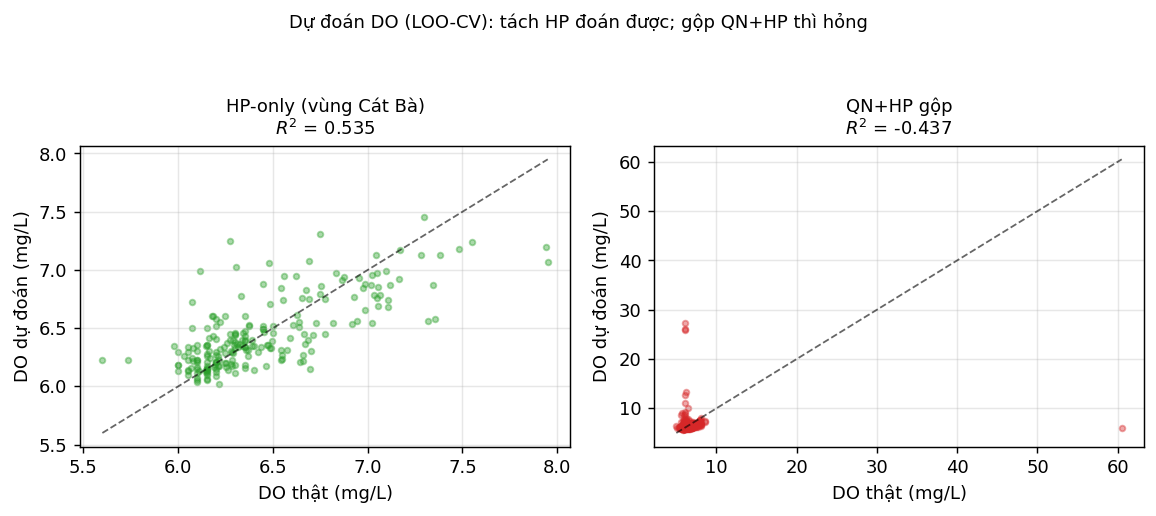
\includegraphics[width=\linewidth]{../figures/do_per_region.png}
    \end{column}
  \end{columns}
  \vspace{2pt}\footnotesize DO Cát Bà \textbf{model-grounded} (mạnh); cùng Salinity (mạnh, cả 2 vùng) + PO4 (yếu). Test: \textbf{37/37 PASS}.
\end{frame}

\begin{frame}{$R^2\approx0{,}999$ là artifact dữ liệu}
  \begin{columns}
    \begin{column}{0.4\textwidth}
      \begin{itemize}\small
        \item BOD5--COD corr $0{,}977$; Alkalinity--COD $0{,}955$.
        \item Điểm bám sát một đường tất định $\Rightarrow$ quan hệ hàm do sinh dữ liệu.
        \item ``Thắng'' của 5-feature phụ thuộc hoàn toàn vào COD --- đúng cảm biến đã chết.
      \end{itemize}
    \end{column}
    \begin{column}{0.6\textwidth}
      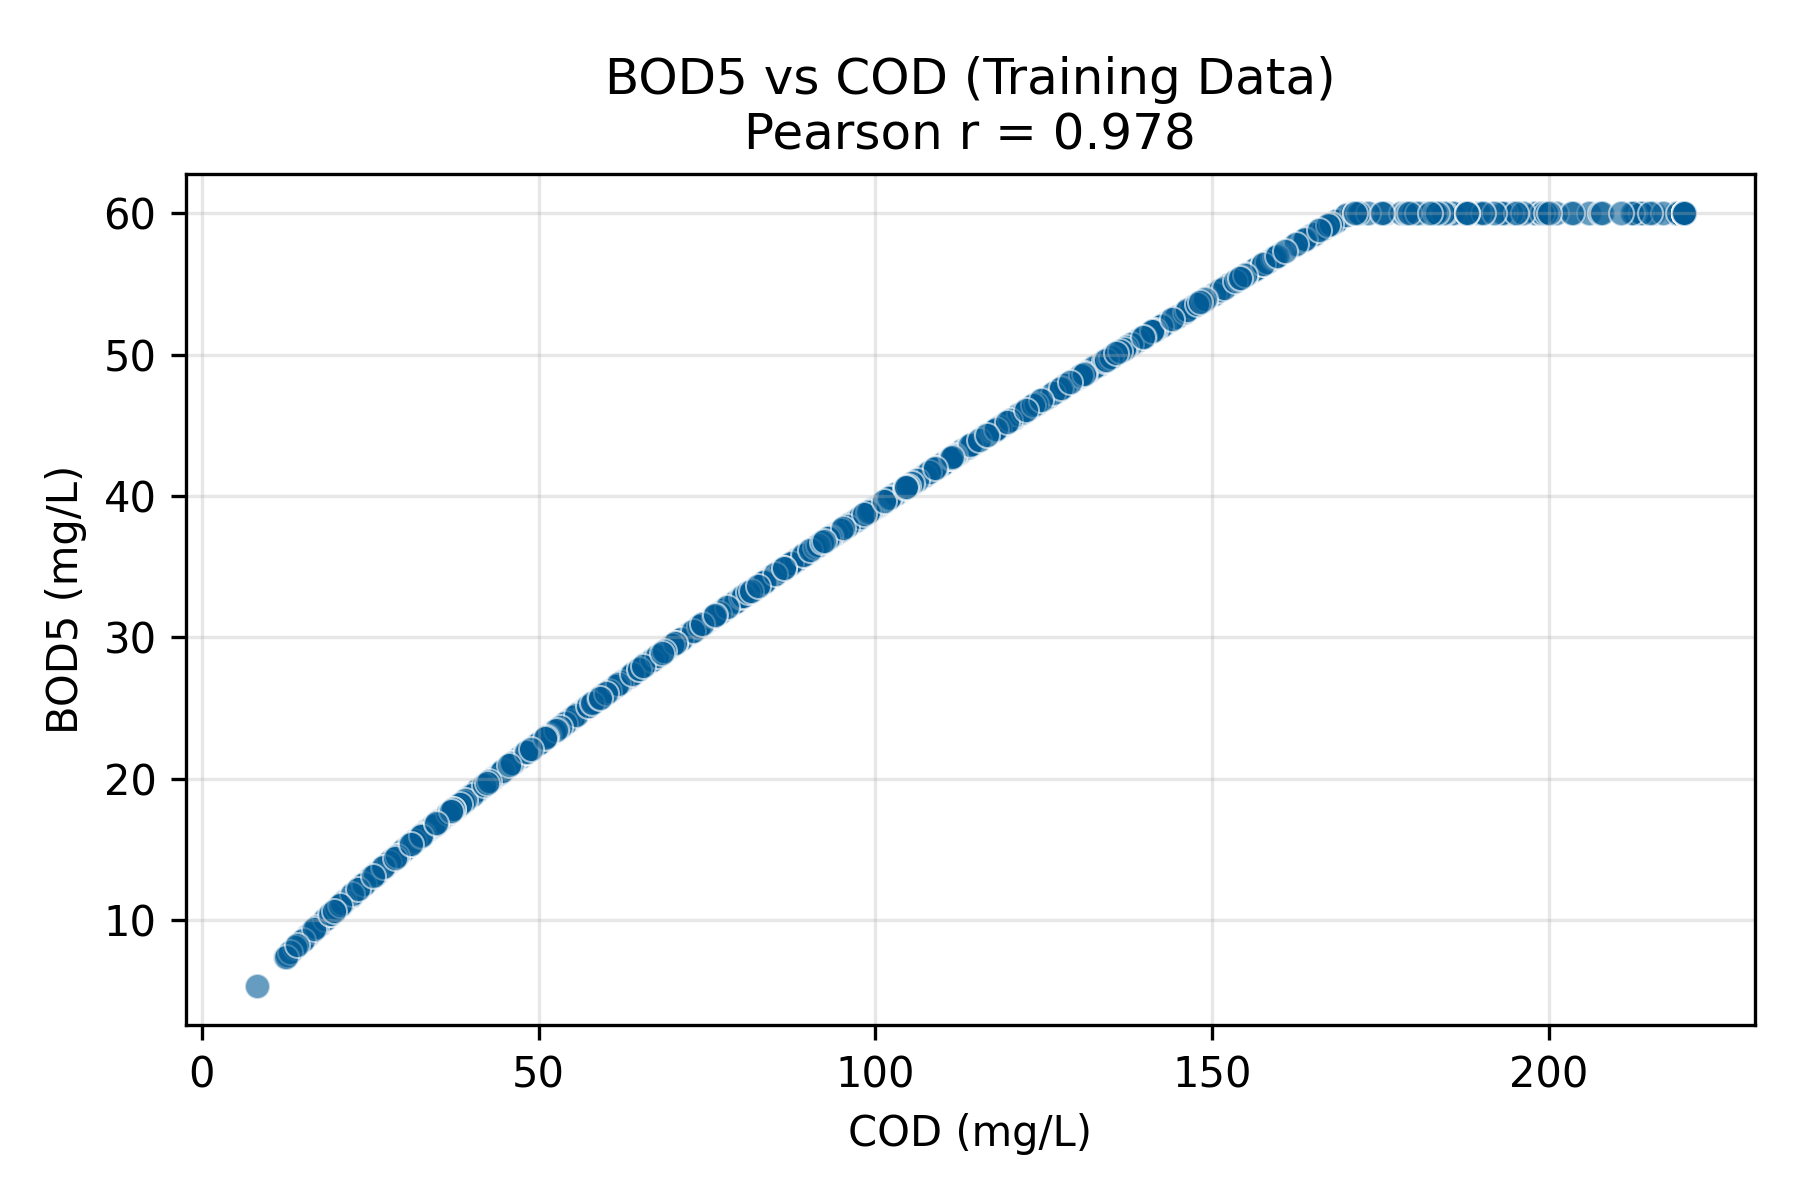
\includegraphics[width=\linewidth]{../figures/bod5_cod_scatter.png}
    \end{column}
  \end{columns}
\end{frame}

% ===================================================================
\section{Hạn chế \& Kết luận}
\begin{frame}{Hạn chế then chốt}
  \begin{itemize}
    \item \textbf{H1:} chính sách 3 mức + Salinity $\to$ Cát Bà có \textbf{3 chỉ số ML-grounded}: DO, Salinity (mạnh) + PO4 (yếu); kim loại/Coliform vẫn trung vị (đã kiểm: không đoán được).
    \item \textbf{H2 (giảm):} nhãn vẫn lệch ``phù hợp'' (0{,}900) vì $\sim$71\% còn là median; nhưng Salinity (top-2) đã hết là hằng số $\to$ bớt chi phối.
    \item \textbf{H3:} $R^2{\approx}0{,}999$ (BOD5/Alkal., chỉ ở QN) là artifact dữ liệu.
    \item \textbf{H4 (đính chính):} DO \emph{đoán được} khi tách HP-only --- ``không đoán được'' trước đó là do gộp sai vùng.
  \end{itemize}
  \vfill
  \begin{block}{Khuyến nghị}
    Phần \textbf{giám sát QCVN} đáng tin. Phần \textbf{phân loại} chỉ là \emph{demo} tới khi: (a) có cảm biến DO + độ muối, (b) sửa COD, (c) xác nhận đơn vị NH4.
  \end{block}
\end{frame}

\begin{frame}{Khả năng lấp 19--20 chỉ số theo loài}
  \begin{columns}[T]
    \begin{column}{0.5\textwidth}
      \footnotesize
      \textbf{Cá giò --- Hải Phòng (Cát Bà)} \\ \textcolor{green!50!black}{\textbf{ĐANG LIVE}} · cần 19 chỉ số
      \begin{itemize}\small
        \item Đo thật + hóa học: pH, Temp, TSS, NH3 (4)
        \item \textbf{ML:} DO + Salinity (mạnh) + PO4 (yếu) (3)
        \item Median: 12 kim loại/Coliform/khác (12)
      \end{itemize}
      $\Rightarrow$ \textbf{đoán được vài chỉ số}, demo chạy được. Tốt nhất trong 2 loài.
    \end{column}
    \begin{column}{0.5\textwidth}
      \footnotesize
      \textbf{Hàu --- Quảng Ninh (Vân Đồn)} \\ \textcolor{red!70!black}{\textbf{CHƯA CÓ DỮ LIỆU SENSOR}} · cần 20 chỉ số
      \begin{itemize}\small
        \item Sensor Vân Đồn \emph{chưa kích hoạt} $\to$ chưa chạy live.
        \item Khi có: QN nội suy được \textbf{Salinity (mạnh)} + Transparency (yếu); nhưng \textbf{DO ở QN $R^2<0$} (không đoán được) --- ngược với HP.
      \end{itemize}
      $\Rightarrow$ \textbf{ưu tiên: triển khai sensor Quảng Ninh} + thêm cảm biến DO (QN không nội suy được).
    \end{column}
  \end{columns}
  \vfill
  \begin{block}{Kết luận}
    Dữ liệu hiện tại (HP) đủ để \textbf{demo cá giò}; muốn làm \textbf{hàu} phải \textbf{bật sensor Quảng Ninh trước} --- và DO/độ muối vẫn cần đo trực tiếp.
  \end{block}
\end{frame}

\begin{frame}{Hướng phát triển}
  \begin{enumerate}
    \item Tích hợp thêm thu thập trạm ở Quảng Ninh, Thái Bình $\to$.
    \item Bổ sung cảm biến DO + độ muối (hai chỉ số đang là hằng số).
    \item Xác nhận đơn vị NH4 với nhà cung cấp.
    % \item Khi đủ chuỗi thời gian: thử dự báo (forecast) thay vì phân loại tức thời.
    % \item Tích hợp phần giám sát QCVN (đã đáng tin) vào webapp.
  \end{enumerate}
\end{frame}

\begin{frame}[plain]
  \centering\vfill
  {\Large Cảm ơn đã lắng nghe}\\[4pt]
  \vfill
\end{frame}

\end{document}
